\documentclass[preprint,12pt,authoryear]{elsarticle}
\usepackage{amssymb}
\usepackage{mathtools}

\journal{Optik}

\begin{document}

\begin{frontmatter}

\title{SILENT - Spectrograph sImuLation and EmulatioN Tool}

\author{Daniel P. Sablowski\thanks{Corresponding author \email{dsablowski@aip.de}}}

\address{Leibniz Institut for Astrophysics Potsdam (AIP), An der Sternwarte 16, D-14482 Potsdam}

\begin{abstract}
We will present a software tool which was designed to compute basic optical parameters of spectrographs. The idea is to find a first
layout of the spectrograph by focusing on the science goal to which the instrument needs to be adapted.  We focus on systems used
in astrophysical instrumentation. These are classical, 3D and echelle spectrograph systems. The code also computes efficiencies of
the specified systems, expected signal-to-noise ratios, layout of the spectral orders on the detector, ect. Furthermore, a complete
frame of the detector can be simulated. This artificial data is used to compare the performance of different designs and to test
data reduction pipelines, before the system is phyisically build. Some additional tools are implemented to characterize special
optical  devices and for the telescope-spectrograph-interface.

\end{abstract}

\begin{keyword}

spectrograph \sep simulation
%% keywords here, in the form: keyword \sep keyword

%% PACS codes here, in the form: \PACS code \sep code

%% MSC codes here, in the form: \MSC code \sep code
%% or \MSC[2008] code \sep code (2000 is the default)

\end{keyword}

\end{frontmatter}

%% \linenumbers

%% main text
\section{Introduction}
\label{Intro}

Since scientific measurements grow in their requirements on precision, it is of great importance to analyze the output of an instrument
prior to physically building it. The common way to do this, is to create artificial data which reflects all know relevant impacts from
the measurement chain. In astrophysical instrumentation this starts at the source, followed by intergalactic and interstellar medium,
earth's atmosphere, telescope, instrument and ends at the digital output of the detector.
Additionally, before performing detailed ray-tracing it is advantageous to compute overall parameters, e.g., spectral resolution, dispersion,
sampling, grating anamorphism, ect., in an fast and ease way. This could already help top rule out designs which would not address the 
science case, the instrument has to be adapted for. 

\textit{SILENT} was designed to help to optical designer to find the correct design and to create realistic artifical data. This data can be
used to inspect the spectral format on the CCD which is particular important for 3D and echelle spectrographs. Furthermore, if the science case
makes clear, that some spectral regions are of more importance than other, it is necessary to design such that these spectral regions are placed
where maximum instrumental throughput is expected. This is especially important for echelle spectrographs, where these features need to be placed
near the blaze maximum. Since all this can be done without taking into account all the details of aberrations and ray-tracing, \textit{SILENT} uses
basic equations to compute all these parameters.

We will first summarize the implemented tools as well as the output created by \textit{SILENT} for the three implemented spectrograph types in Sect 2.
Sect. 3 is reseved for a design example of an echelle spectrograph. The conclusion and discussion follows in the last Sect. 4.

\section{Tools and Computed Parameters}

In this section we want to give an overview of the implemented tools. We do not show all the calculations in detail, but we give the most important ones. The central equation is the
equation for the diffraction grating

\begin{equation}
 \label{Eq1}
 \frac{n \lambda}{g} = sin(\alpha) + sin(\beta),
\end{equation}
where $n$ is the diffraction order, $\lambda$ the wavelength, $g$ the grating constant, $\alpha$ and $\beta$ the angles of incidence and diffraction, respectively.
Differentiating this equation with respect to the angle of diffraction, we get
\begin{equation}
 \label{Eq2}
 \frac{d\lambda}{d\beta}=\frac{g cos(\beta)}{n}
\end{equation}
the angular dispersion. And we get the linear dispersion per pixel on the CCD
\begin{equation}
 \label{Eq3}
 D=\frac{p B g cos(\beta)}{f_{cam} n}
\end{equation}
when we use the focal length of the imaging camera $f_{cam}$, the size of a pixel in the direction of dispersion $p$ and the binning factor $B$ on the CCD
The two-pixel resolution is hence given by $d\lambda_{2p}=2D$. In a similar way (Differentiating with respect to $\alpha$) we get the non-pixel-limited 
resolving power to
\begin{equation}
 \label{Eq4}
 \frac{\lambda}{d\lambda}=f_{coll}\frac{n \lambda}{b g cos(\alpha)}a,
\end{equation}
where $a=cos(\alpha)/cos(\beta)$ is the anamorphism of the grating, $b$ the width of the input slit and $f_{coll}$ the focal length of the collimating optics.
The Nyquist factor is defined as
\begin{equation}
 \label{Eq5}
 N \equiv \frac{b'}{2p}
\end{equation}
the ratio between the size of the imaged slit width $b' = b a f_{cam}/f_{coll}$ and the size of two pixels and it should be greater than unity. These
geometrical spectral parameters are computed by \textit{SILENT} and written to a local file.

Additionally, the program computes efficiency data. We use an analytical approximation for the blaze function and the user is free to set the peak value.
The number of present optical surfaces is specified and will be interpolated for the computed wavelength points. The data can be easily replaced by custom
data which should be provided by the manufacturer.

\subsection{The classical spectrograph}

All standard designs (Littrow, Czerny-Turner, etc.) with one diffraction element fall into this category. We have implemented standard diffraction grating
and volume-phase-holographic (VPH) grating as options for the diffraction element. In Fig. \ref{Fig1} we show a CCD frame of 2048 x 1024 pixels with
a Balmer absorption continuum. We have also applied an image slicer which generates the six spectra visible. 

\begin{figure}[]
 \begin{center}
 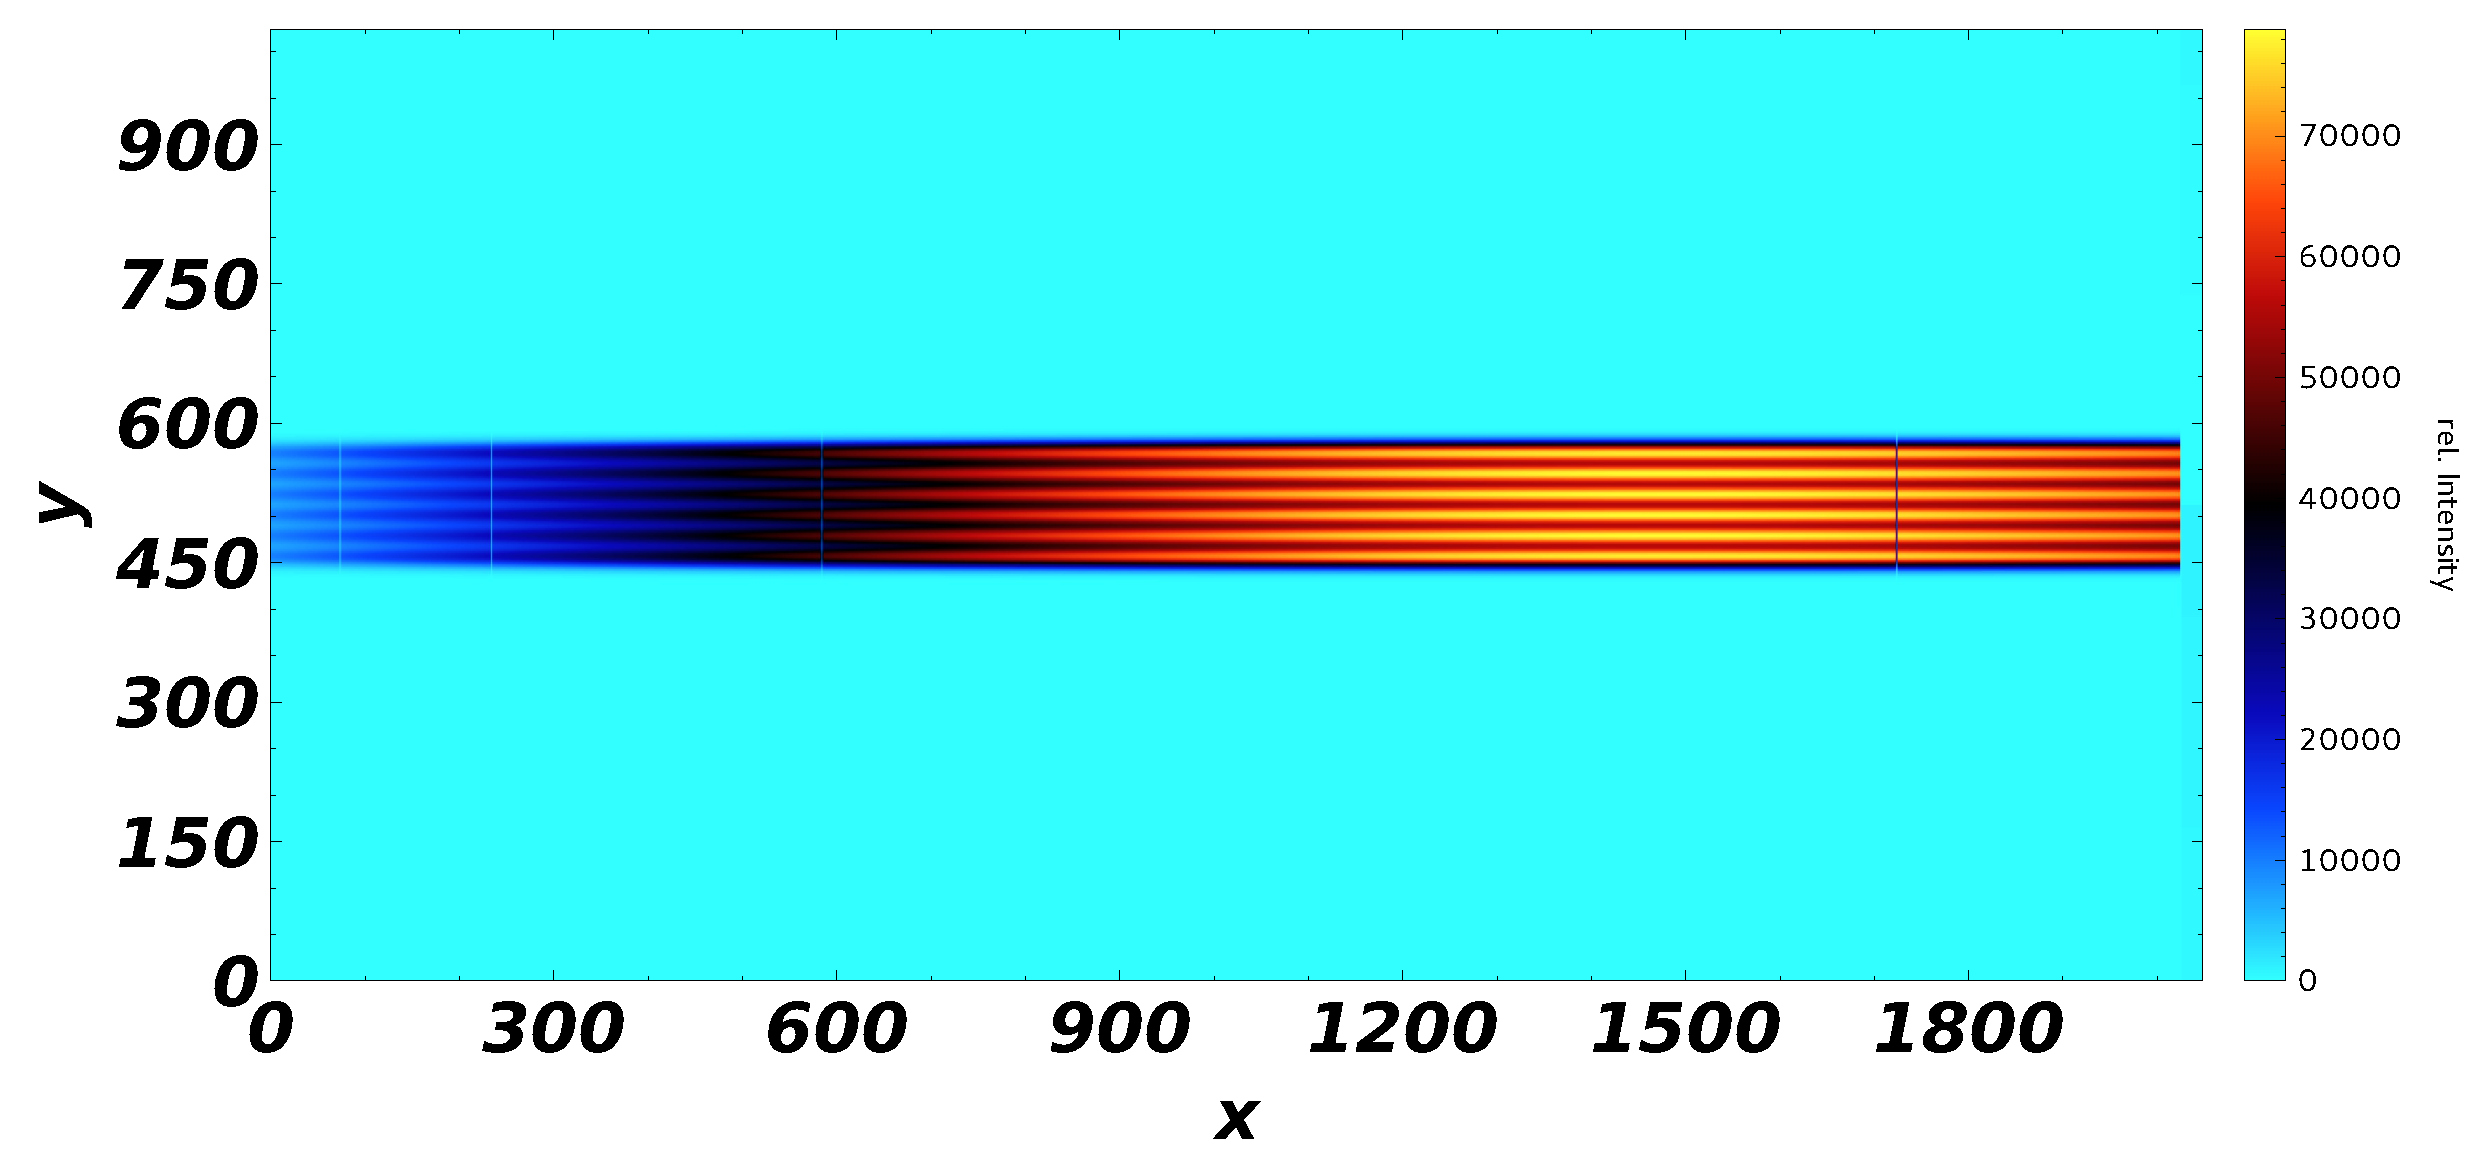
\includegraphics[trim=0cm 0cm 4cm 0cm, clip=true, width=120mm]{./clbalmer.pdf}
 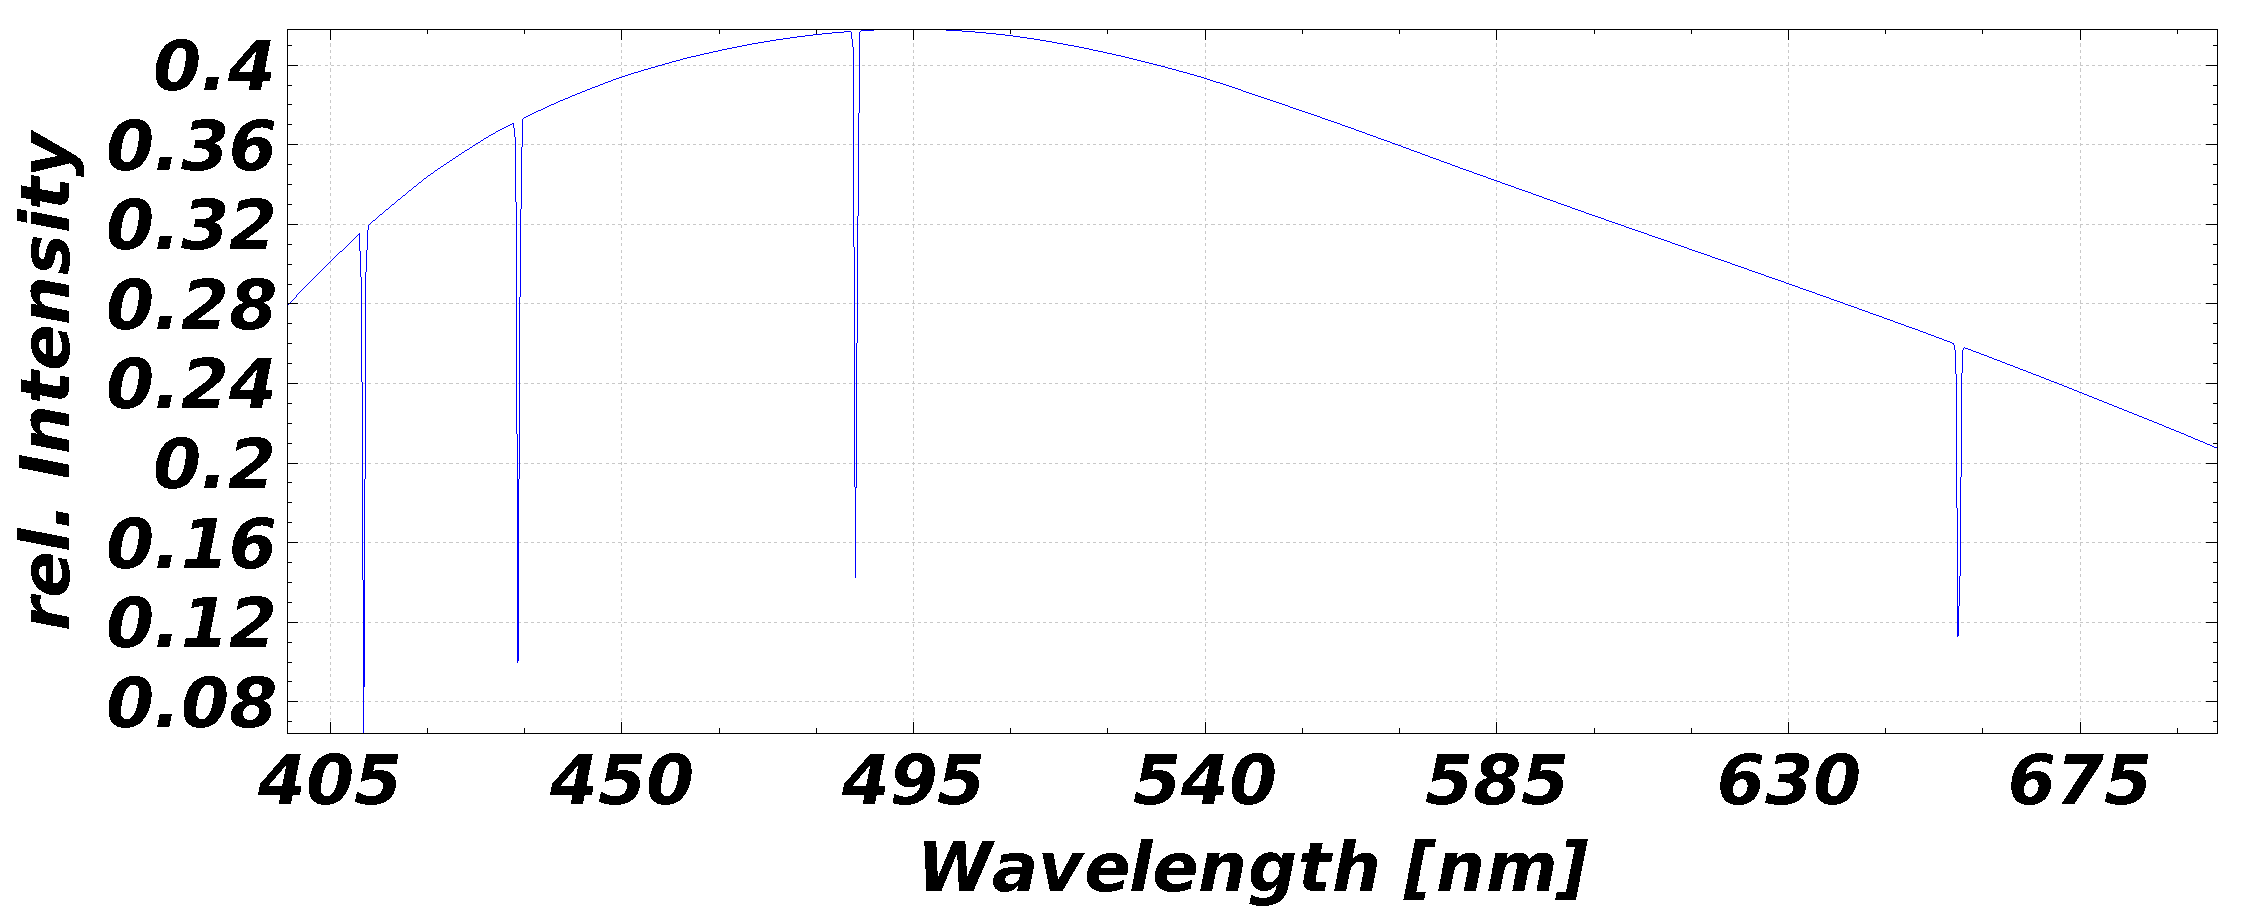
\includegraphics[width=120mm]{./clspec.pdf}
\end{center}
 \caption{}
  \label{Fig1}
  \end{figure}

\subsection{The echelle spectrograph}

\subsection{The 3D spectrograph}

\subsection{additional tools}

\section{A Design Example}

\section{Conclusion and Discussion}

%% The Appendices part is started with the command \appendix;
%% appendix sections are then done as normal sections
%% \appendix

%% \section{}
%% \label{}

%% If you have bibdatabase file and want bibtex to generate the
%% bibitems, please use
%%
%%  \bibliographystyle{elsarticle-harv} 
%%  \bibliography{<your bibdatabase>}

%% else use the following coding to input the bibitems directly in the
%% TeX file.

\begin{thebibliography}{00}

%% \bibitem[Author(year)]{label}
%% Text of bibliographic item

\bibitem[ ()]{}

\end{thebibliography}
\end{document}

\endinput
%%
%% End of file `elsarticle-template-harv.tex'.
